%!TEX root = ../dissertation.tex
\begin{savequote}[75mm]
A good idea is about ten percent and implementation and hard work, and luck is 90 percent.
\qauthor{Guy Kawasaki}
\end{savequote}

\chapter{Implementation}
This chapter is about the implementation with Apache Storm to solve the defined queries and to do the benchmarks.
The idea of the test scenario is to use "OSM Augmented Diffs" as a stream.
This diffs extend the ordinary minutely diffs of OSM with more information.
The result contains all the nodes, ways and relations changed durring the time periode.

\newpage

\section{Test Setup}
For the implementation there is a given test setup.
The Open Street Map Augmented diffs are minutelly collected by a script executed as a cron job.
The script acts as an producer for Kafka and the data is now accessible from these message queue.
Furthermore the data is ready to be consumed by the stream processing engine and in this case ready for Apache Storm.

\begin{figure}[H]
\centering
\captionsetup{justification=centering}
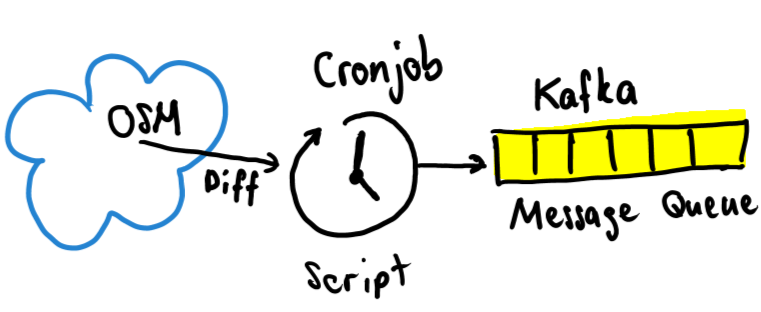
\includegraphics[width=0.6\textwidth]{images/test_setup.png}
\caption[Test setup]{Test setup}
\end{figure}


\section{Queries}
The following list is about the queries which has to be done on the Augmented Diff stream.

\begin{itemize}
\item[A)] Leader board of top 10 OSM active users
\item[B)] Leader board of top 10 OSM objects added
\item[C)] Node objects with suspicious keys and values
\item[D)] Way objects with only user tag "area=yes" without other user tags
\end{itemize}

\subsection{A) Leader board of top 10 OSM active users}
It's about users who created or updated any OSM nodes all around the world.
The users are identified by the tags "uid" and "user".

\subsection{B) Leader board of top 10 OSM objects added}
Count all the created or updated nodes grouped by a combination of key and value.
An example for this is "amenity=bench".

\subsection{C) Node objects with suspicious keys and values}
Detection of vandalism and unwanted bad actions in OpenStreetMap is a very difficult topic.
Thus we focus on "Quality Assurance Monitoring" by filtering for suspicious tags of node or way elements.
As an example for this issues are ";" in Tags like "crossing=island;uncontrolled".

\subsection{D) Way objects with only user tag "area=yes" without other user tags}
The point D) also deals with the vandalism problems.


\newpage
\section{Topic of the queries}


\newpage
\section{Benchmark}

Benchmarking is a very difficult topic and strongly depends on various parameters like the underlying hardware.
Thus we decide to make this as hardware independent as possible.
The idea is to produce a lot of small kafka message, like IoT does,
and to count them. Then repeat this process and relate the number of processed messages with the time spent.

For the message generation we had a small python script called "benchmark.py" which produces as much massages as you want
and stores them in to kafka.

The messages have got the following structure:

   \begin{table}[h!]
     \centering
     \begin{tabular}{llllll}
       \textbf{packetId}  & \textbf{TopicName} & \textbf{qos} & \textbf{retainFlag} & \textbf{payload} & \textbf{dupFlag} \\
       0 & weather & 5 & False & 83 & True \\
       1 & computer & 2 & True & 82 & False \\
     \end{tabular}
     \caption{MQTT Messages}
     \label{MQTT Messages}
   \end{table}

To realize the benchmark with apache storm I tried two different topics.
The first with only one Bolt, which is the non parallelism way. This leads to the blue curve on the diagramm.
\begin{figure}[H]
\centering
\captionsetup{justification=centering}
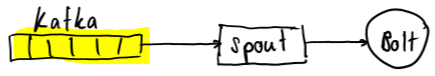
\includegraphics[width=0.4\textwidth]{images/benchmark_topic1.png}
\caption[Benchmark 1 Bolt]{Benchmark 1 Bolt}
\end{figure}

For the second approach I use four Bolts for parallelism.
The decision for four Bolts depends on the four cores of the notebook which I used for the benchmarks.
The result is the red curve on the diagramm.

\begin{figure}[H]
\centering
\captionsetup{justification=centering}
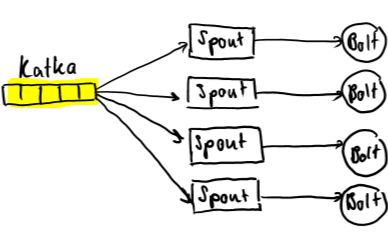
\includegraphics[width=0.4\textwidth]{images/benchmark_topic2.png}
\caption[Benchmark 4 Bolts]{Benchmark 4 Bolts}
\end{figure}


\begin{figure}[H]
\centering
\captionsetup{justification=centering}
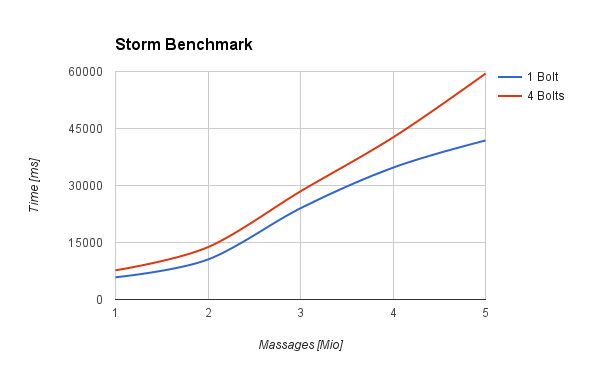
\includegraphics[width=1.0\textwidth]{images/benchmark.png}
\caption[Benchmark Diagramm]{Benchmark Diagramm}
\end{figure}

\subsection{Conclusion}
To take a good conclusion out of this benchmark is a hard tasks.
On the one hand side it's no problem for storm to process millions of messages.
But on the other hand side I couldn't perform better with more messages. It was more or less a linear behavior.
An a bit unsuspected was that the parallelism topic was slower than to work with only one Bolt.
Maybe this behavior would change with bigger messages.
I think the bottleneck in the construction was the communication with kafka. And so the throughput was limited by the networking.





